\documentclass[14pt,aspectratio=169]{beamer}

\usepackage{pgfpages}
\usepackage{fancyvrb}

\usepackage{tikz}
\usepackage{pgfplots}

\usepackage{minted}
\usemintedstyle{tango}

\usepackage{graphicx}

\usetheme{auriga}
\usecolortheme{auriga}

\setbeamercolor{background canvas}{bg=lightgray}

% define some colors for a consistent theme across slides
\definecolor{red}{RGB}{181, 23, 0}
\definecolor{blue}{RGB}{0, 118, 186}
\definecolor{gray}{RGB}{146, 146, 146}

\title{Web Development: \\ Programming in CSS}

\author{{\bf Gregory M. Kapfhammer}}

\institute[shortinst]{{\bf Department of Computer Science, Allegheny College}}

\begin{document}

{
  \setbeamercolor{page number in head/foot}{fg=background canvas.bg}
  \begin{frame}
    \titlepage
  \end{frame}
}

%% Slide
%
\begin{frame}{Technical Question}
  %
  \hspace*{.25in}
  %
  \vspace*{.1in}
  %
  \begin{center}
    %
    {\large How can I follow industry best practices for implementing syntactically valid
      cascading style sheets (CSS) files that correctly use selectors, properties,
    and media queries to modify the display of text-based and image content?}
    %
  \end{center}
  %
  \vspace{1ex}
  %
  \begin{center}
    %
    \small Let's learn more about how to use CSS to write useful style sheets!
    %
  \end{center}
  %
\end{frame}

% Slide
%
\begin{frame}{Web Pages with HTML and CSS Code}
%
  \begin{itemize}
    %
    \item CSS stands for the language for cascading style sheets
      %
    \item HTML and CSS are major components of the modern web
      \begin{itemize}
        \item Markdown, HTML, CSS, JavaScript
        \item Design, implementation, and testing
        \item Deployment, maintenance, monitoring
        \item Linting and testing tools for all languages
      \end{itemize}
      %
    \item What are the style sheets described as ``cascading''?
      %
  \end{itemize}
%
\end{frame}

% Slide
%
\begin{frame}{Correctly Using Both HTML and CSS}
%
  \begin{itemize}
    %
    \item HTML should not handle formatting or presentation
      %
      \vspace*{-.2in}
      %
    \item CSS can describe the appearance of HTML elements
      %
      \vspace*{-.15in}
      %
    \item Benefits of using CSS to style elements
      \begin{itemize}
        \item Improved control over formatting
        \item Improved site maintainability
        \item Improved accessibility
        \item Improved page download speed
        \item Improved output flexibility
      \end{itemize}
      %
      \vspace*{-.2in}
      %
    \item CSS enables {\em mobile-ready} or {\em responsive} web pages
  \end{itemize}
%
\end{frame}

% Slide
%
\begin{frame}{Versions and Adoption of CSS}
%
  \begin{itemize}
    %
    \item Distinction between {\em data} and {\em meta-data} and {\em style}
      %
      \vspace*{-.1in}
      %
    \item Versions and adoption of CSS
      \begin{itemize}
        \item Should style be expressed in JavaScript?
        \item Should style be expressed by key value pairs?
        \item Should styling involve colors and fonts?
        \item How should web page styling be organized?
      \end{itemize}
      %
      \vspace*{-.2in}
      %
    \item Check sites like \url{https://caniuse.com/} to learn more about the
      current features of CSS3 and its browser support. Different browsers have
      different support!
      %
  \end{itemize}
%
\end{frame}

% Slide
%
\begin{frame}{Syntax and Semantics of CSS}
%
  \begin{itemize}
    %
    \item A {\em selector} identifies a matching HTML element
      %
      \vspace*{-.2in}
      %
    \item Key-value pairs define properties associated with values
      %
      \vspace*{-.15in}
      %
    \item Summary of the components in CSS files
      \begin{itemize}
        \item Selectors
        \item Properties
        \item Values
        \item Organized into style sheets
        \item Located in three different places
      \end{itemize}
      %
      \vspace*{-.2in}
      %
    \item CSS content can be {\em inline} or {\em embedded} or {\em external} to web pages.
      What are the trade-offs in these approaches?
  \end{itemize}
%
\end{frame}

% Slide
%
\begin{frame}[fragile]
  \frametitle{Programming CSS: Using Key-Value Pairs}
  \normalsize
  \hspace*{.25in}
  \begin{minipage}{6in}
    \vspace*{.2in}
    \begin{minted}[mathescape, numbersep=5pt, fontsize=\large]{css}
th {
  font-weight: bold;
}
td {
  text-align: center;
}
    \end{minted}
  \end{minipage}
  \vspace*{.05in}
  \begin{center}
    %
    \noindent What are the HTML tags that this selector styles?\\
    \noindent Can you find the key value pairs in this CSS code?\\
    %
  \end{center}
  %
\end{frame}

% Slide
%
\begin{frame}[fragile]
  \frametitle{Programming CSS: Changing Color and Size}
  \normalsize
  \hspace*{.25in}
  \begin{minipage}{6in}
    \vspace*{.2in}
    \begin{minted}[mathescape, numbersep=5pt, fontsize=\large]{css}
table {
  color: #333;
  width: 600px;
}
    \end{minted}
  \end{minipage}
  \vspace*{.05in}
  \begin{center}
    %
    \noindent What is the HTML tag that the selector styles?\\
    \noindent Can you find the key value pairs in this CSS code?\\
    \noindent What is the meaning of {\tt \#333}? What is the meaning of {\tt 600px}?\\
    %
  \end{center}
  %
\end{frame}

% Slide
%
\begin{frame}[fragile]
  \frametitle{Programming CSS: Changing Table Borders}
  \normalsize
  \hspace*{.25in}
  \begin{minipage}{6in}
    \vspace*{.2in}
    \begin{minted}[mathescape, numbersep=5pt, fontsize=\large]{css}
table {
  border: solid #777;
  border-width: 1pt 0pt 0pt 1pt;
  border-spacing: 0;
}
    \end{minted}
  \end{minipage}
  \vspace*{.05in}
  \begin{center}
    %
    \noindent What is the HTML tag that this selector styles?\\
    \noindent Can you find the key value pairs in this CSS code?\\
    %
    \noindent What is the meaning of {\tt \#777}? What is the meaning of {\tt
    1pt} or {\tt 0pt}? What does it mean if there is a number with no unit?\\
    %
  \end{center}
  %
\end{frame}

% Slide
%
\begin{frame}{Interaction Among Different CSS Styles}
  %
  \begin{itemize}
    %
    \item How do we know which CSS rule to apply to an HTML element? Sometimes
      it can be tricky! Try it out!
      %
      \vspace*{-.2in}
      %
    \item {\bf Styles}: author-created, user-defined, default browser
      %
      \vspace*{-.15in}
      %
    \item The ``cascading principles'' a browser follows:
      %
      \begin{itemize}
        %
        \item {\bf Inheritance}: Property affects HTML element and its
          descendants
          %
        \item {\bf Specificity}: More specific selector has more precedence
          %
        \item {\bf Location}: The most recent rules in a file have precedence
          %
      \end{itemize}
      %
      \vspace*{-.2in}
      %
    \item What about the use of the {\tt !important} decorator in CSS files?
      Please use a browser's web development tools!
      %
  \end{itemize}
  %
\end{frame}

% Slide
%
\begin{frame}{The CSS Box Model}
  %
  \begin{itemize}
    %
    \item How do we style the various ``boxes'' that exist inside of a web
      page? What are these boxes? One example: {\tt <div>}
      %
      \vspace*{-.2in}
      %
    \item The attributes of an HTML element's box:
      %
      \begin{itemize}
        %
        \item {\bf Border}: the box surround all sides of an element
          %
        \item {\bf Margin}: the space outside the border around an element
          %
        \item {\bf Padding}: The space inside of the border around the element
          %
        \item {\bf Height}: how tall is the inner box of an element
          %
        \item {\bf Width}: how wide is the inner box of an element
          %
        \item {\bf Background}: what is the color or image of an element
          %
      \end{itemize}
      %
      \vspace*{-.2in}
      %
    \item Use a browser's web development tools to see the CSS3 box model and
      to interact with styles. {\bf Remember TRBL}!
      %
  \end{itemize}
  %
\end{frame}

% Slide
%
\begin{frame}[fragile]
  \frametitle{Exploring the Box Model in CSS: Paragraphs}
  \normalsize
  \hspace*{.25in}
  \begin{minipage}{6in}
    \vspace*{.2in}
    \begin{minted}[mathescape, numbersep=5pt, fontsize=\large]{css}
p,
ul {
  border: 2px solid rebeccapurple;
  padding: .5em;
}
    \end{minted}
  \end{minipage}
  \vspace*{.05in}
  \begin{center}
    %
    \noindent What are the HTML tags that this selector styles? \\
    %
    \noindent Hey, the CSS rules apply to two HTML tags! \\
    %
    \noindent Can you find the key value pairs in this CSS code? \\
    %
  \end{center}
  %
\end{frame}

% Slide
%
\begin{frame}[fragile]
  \frametitle{Exploring the Box Model in CSS: List Items}
  \normalsize
  \hspace*{.25in}
  \begin{minipage}{6in}
    \vspace*{.2in}
    \begin{minted}[mathescape, numbersep=5pt, fontsize=\large]{css}
.block,
li {
  border: 2px solid blue;
  padding: .5em;
}
    \end{minted}
  \end{minipage}
  \vspace*{.05in}
  \begin{center}
    %
    \noindent What are the HTML tags that this selector styles? \\
    %
    \noindent Hey, the CSS rules apply to two HTML tags! \\
    %
    \noindent Can you find the key value pairs in this CSS code? \\
    %
  \end{center}
  %
\end{frame}

% Slide
%
\begin{frame}[fragile]
  \frametitle{Using CSS to Assign ``Flex'' to HTML Elements}
  \normalsize
  \hspace*{.25in}
  \begin{minipage}{6in}
    \vspace*{.2in}
    \begin{minted}[mathescape, numbersep=5pt, fontsize=\large]{css}
ul {
  display: flex;
  list-style: none;
}
    \end{minted}
  \end{minipage}
  \vspace*{.05in}
  \begin{center}
    %
    \noindent What are the HTML tags that this selector styles? \\
    %
    \noindent Can you find the key value pairs in this CSS code? \\
    %
    \noindent What is the meaning of {\tt display: flex;}? \\
    %
  \end{center}
  %
\end{frame}

% Slide
%
\begin{frame}[fragile]
  \frametitle{Controlling the Display of Content with CSS}
  \normalsize
  \hspace*{.25in}
  \begin{minipage}{6in}
    \vspace*{.2in}
    \begin{minted}[mathescape, numbersep=5pt, fontsize=\large]{css}
.block {
  display: block;
}
    \end{minted}
  \end{minipage}
  \vspace*{.05in}
  \begin{center}
    %
    \noindent What is the HTML tag that this selector styles? \\
    %
    \noindent Can you find the key value pairs in this CSS code? \\
    %
    \noindent What is the meaning of {\tt display: block;}? \\
    %
    \noindent HTML elements are either {\em block} or {\em inline}! \\
    %
  \end{center}
  %
\end{frame}

% Slide
%
\begin{frame}[fragile]
  \frametitle{Connecting CSS Rules to HTML Content}
  \normalsize
  \hspace*{.15in}
  \begin{minipage}{6in}
    \vspace*{.2in}
    \begin{minted}[mathescape, numbersep=5pt, fontsize=\small]{html}
<p>I am a paragraph. A short one.</p>
<ul>
  <li>Item One</li>
  <li>Item Two</li>
  <li>Item Three</li>
</ul>
<p>I am another paragraph.
Some of the <span class="block">words</span>
have been wrapped in a <span>span element</span>.</p>
    \end{minted}
  \end{minipage}
  \vspace*{.05in}
  \begin{center}
    %
    \noindent What is the meaning of {\tt class="block"}? \\
    %
    \noindent  \url{https://developer.mozilla.org/en-US/docs/Learn/CSS/Building_blocks/The_box_model}
    %
  \end{center}
  %
\end{frame}

% Slide
%
\begin{frame}{Revisiting the CSS Box Model}
  %
  \begin{itemize}
    %
    \item Reviewing the attributes of an HTML element's box:
      %
      \begin{itemize}
        %
        \item {\bf Border}: the box surround all sides of an element
          %
        \item {\bf Margin}: the space outside the border around an element
          %
        \item {\bf Padding}: The space inside of the border around the element
          %
        \item {\bf Height}: how tall is the inner box of an element
          %
        \item {\bf Width}: how wide is the inner box of an element
          %
        \item {\bf Background}: what is the color or image of an element
          %
      \end{itemize}
      %
      \vspace*{-.2in}
      %
    \item Make sure to distinguish between {\em padding} and {\em margin}!
      %
      \vspace*{-.2in}
      %
    \item Remember TRBL! What do browser's dev tools look like? How do
      you use them during development and debugging?
      %
  \end{itemize}
  %
\end{frame}

\begin{frame}{Using Dev Tools in Chrome}
  %
  \begin{figure}
    \centering
    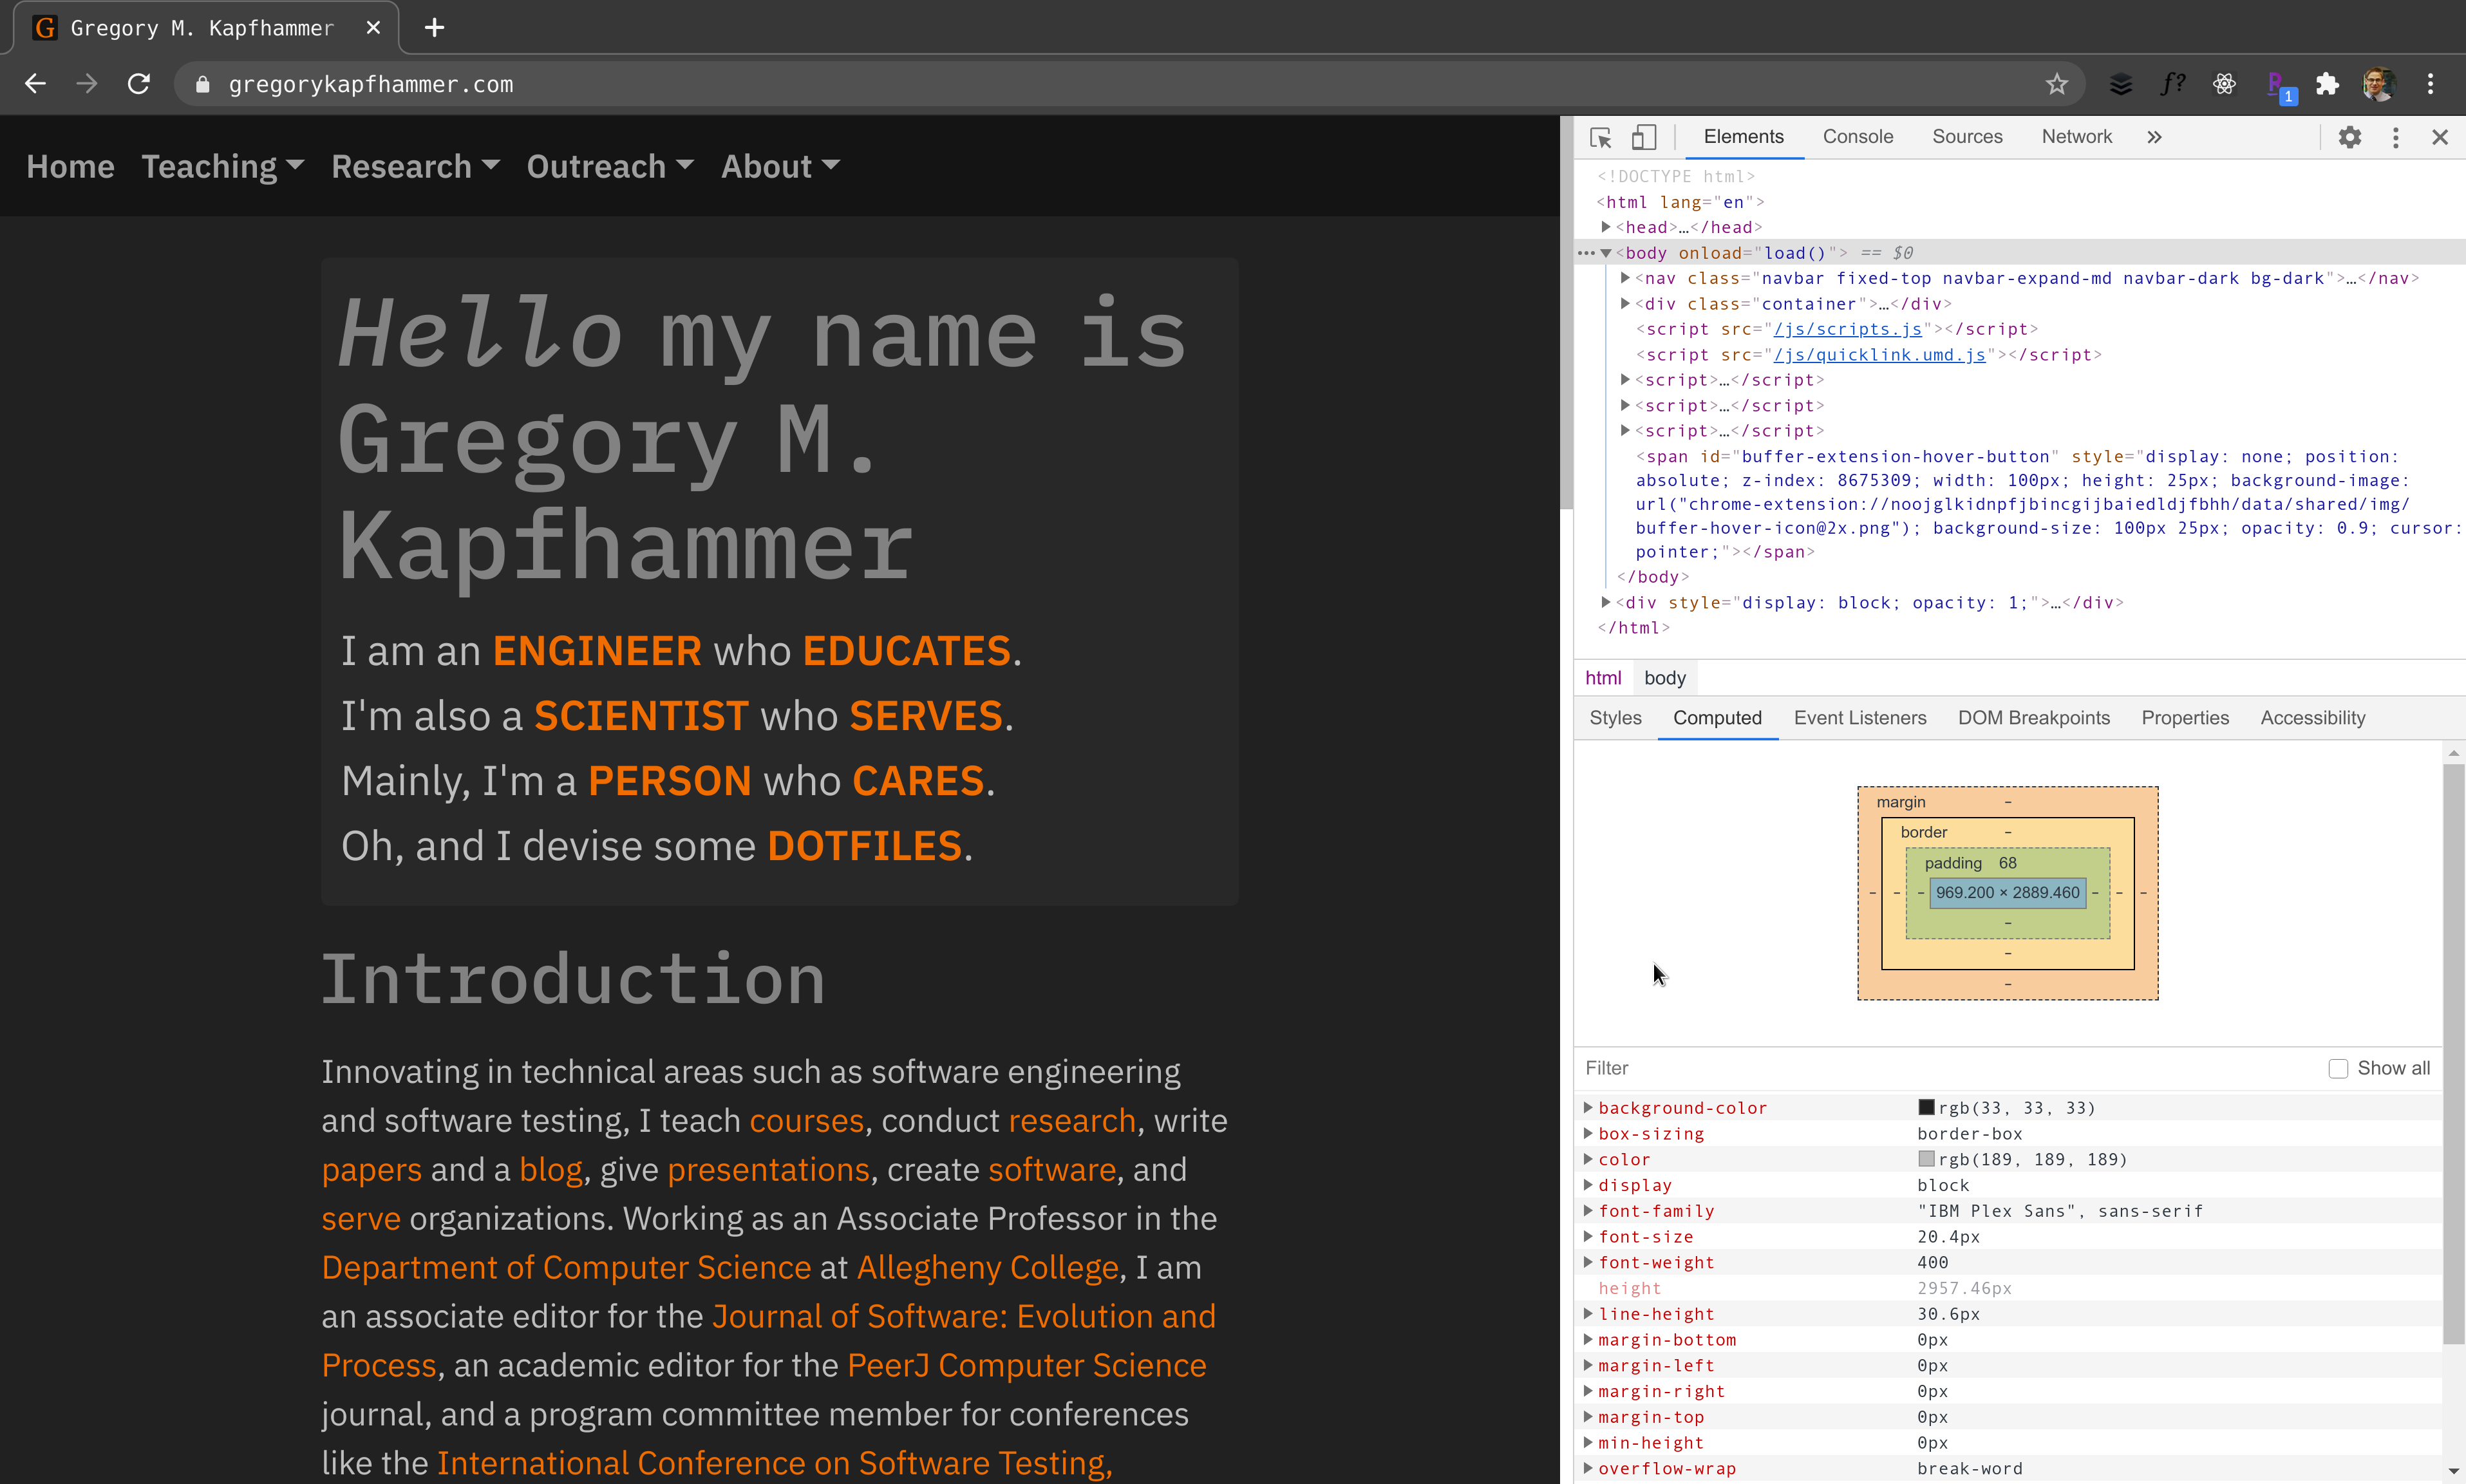
\includegraphics[scale=.085]{images/chrome-dev-tools.png}
    \caption{The figure's caption}
  \end{figure}
  %
\end{frame}
\end{document}
